\section{1174096 - Nico Ekklesia Sembiring}
\subsection{Soal Teori}
\begin{enumerate}

	\item Jelaskan dengan ilustrasi gambar sendiri apa perbedaan antara vanilla GAN dan cGAN.
	\hfill\break
    Perbedaan Vanilla GANs dan cGAN adalah sebagai berikut :
    \hfill\break
    Vanilla GANs biasanya tidak memiliki convolutional Neural Jaringan (CNNs) di jaringan mereka.
    \hfill \break
    Conditional GANs (cGANs) adalah perpanjangan dari model GAN. Mereka memungkinkan untuk generasi gambar yang memiliki kondisi tertentu atau atribut dan telah terbukti menjadi lebih baik dari Vanilla GANs sebagai hasilnya. \\
    cGANs adalah jenis GAN yang dikondisikan pada beberapa informasi tambahan.  informasi tambahan ke Generator sebagai lapisan input tambahan. Dalam Vanilla GANs, tidak ada kontrol atas Kategori gambar yang dihasilkan. Ketika kita menambahkan kondisi y ke Generator, kita dapat menghasilkan gambar dari kategori tertentu, menggunakan y, yang mungkin jenis data, seperti label kelas atau data integer. Vanilla GANs bisa belajar hanya satu kategori dan sangat sulit untuk arsitek GANs untuk beberapa kategori. Sebuah cGAN, bagaimanapun, dapat digunakan untuk menghasilkan model multi-modal dengan kondisi yang berbeda untuk kategori yang berbeda.
    \hfill \break
    \begin{figure}[H]
	\centering
		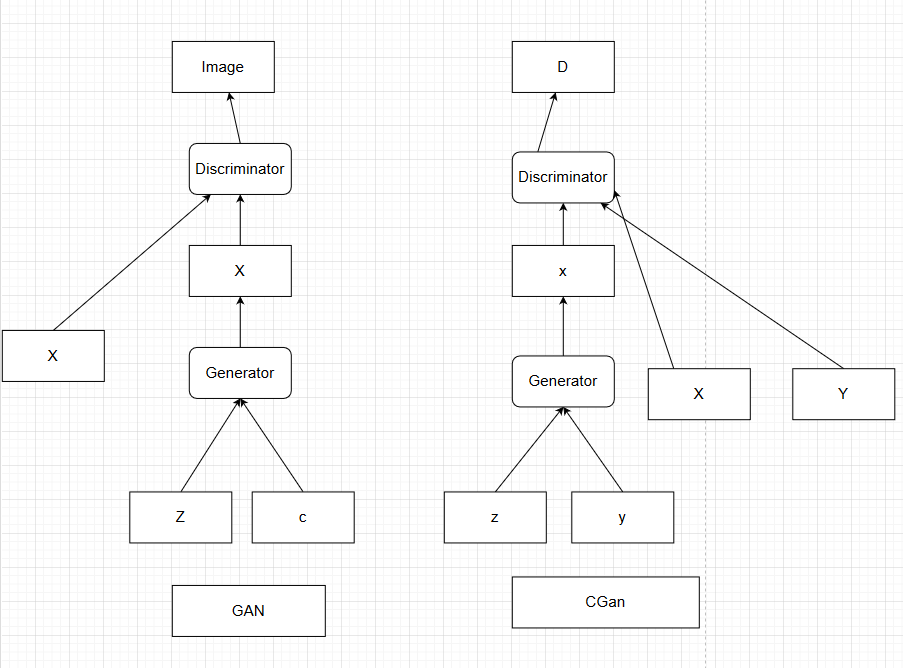
\includegraphics[width=4cm]{figures/1174096/tugas9/teori1.PNG}
		\caption{Ilustrasi Vanilla GANs dan cGAN}
	\end{figure}

	\item Jelaskan dengan ilustrasi gambar sendiri arsitektur dari Age-cGAN.
    \hfill\break
    Age cGan melakukan input sesuai dengan wajah beserta umur. Lalu akan dilakukan proses encoding dan selanjutnya melakukan Optimasi identitas. Lalu dihasilkan rekonstruksi awal yang nanti dilanjutkan dengan generator yang mengoptimasi rekonstruksi.
    \begin{figure}[H]
	\centering
		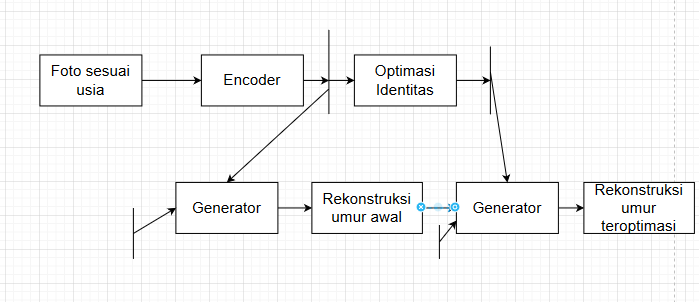
\includegraphics[width=4cm]{figures/1174096/tugas9/teori2.PNG}
		\caption{ilustrasi Age-cGAN}
	\end{figure}

	\item Jelaskan dengan ilustrasi gambar sendiri arsitektur encoder network dari AgecGAN.
	\hfill\break
	Encoder network pada Age cGAN menghasilkan vektor dari gambar yang dimasukkan. Encoder network sendiri merupakan sebuah CNN yang mengambil gambar dengan dimensi sekitar 64,64,3 dan mengkonversikannya menjadi vektor dengan dimensi 100
    \begin{figure}[H]
        \centering
            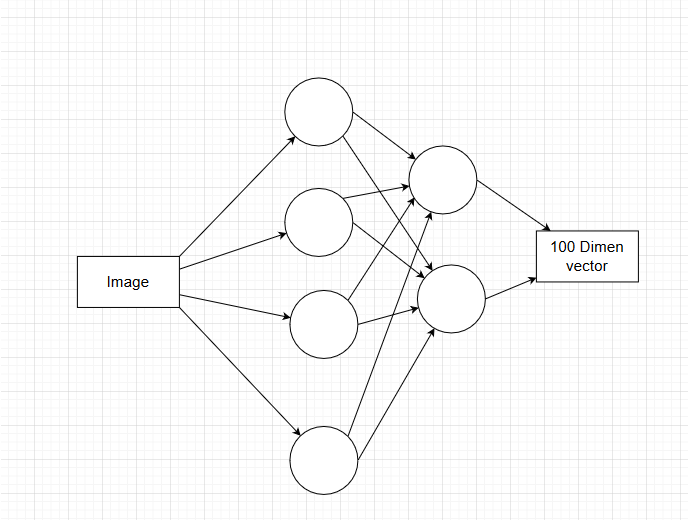
\includegraphics[width=4cm]{figures/1174096/tugas9/teori3.PNG}
            \caption{Ilustrasi arsitektur encoder AgecGAN}
        \end{figure}

	\item Jelaskan dengan ilustrasi gambar sendiri arsitektur generator network dari AgecGAN
	\hfill\break
	Generator network digunakan mengambil representasi yang tersembunyi dari fotowajah dan kondisi vektor sesuai dengan kondisi yang ada. Generator network sendiri memiliki vektor 100 dimensi dan kondisi vektor Y. 
    \begin{figure}[H]
	\centering
		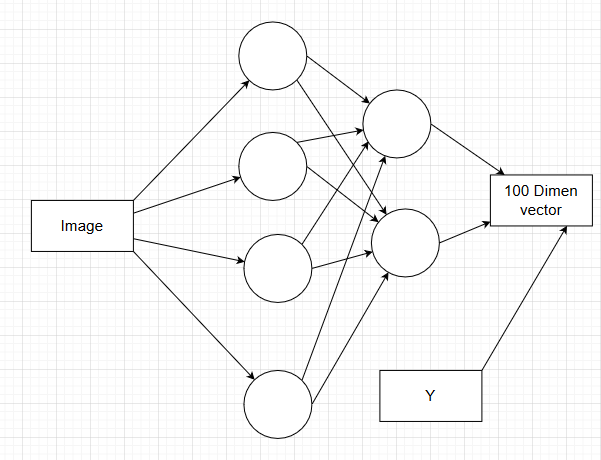
\includegraphics[width=4cm]{figures/1174096/tugas9/teori4.PNG}
		\caption{ilustrasi arsitektur generator network AgecGAN}
	\end{figure}

	\item Jelaskan dengan ilustrasi gambar sendiri arsitektur discriminator network dari Age-cGAN.
	\hfill\break
	jaringan diskriminator digunakan untuk mengidentifikasi apakah gambar yang disediakan adalah palsu atau nyata. Hal ini dilakukan dengan melewati gambar melalui serangkaian lapisan sampling bawah dan beberapa lapisan klasifikasi. Dengan kata lain, ini memprediksi Apakah gambar itu nyata atau palsu. Seperti jaringan lain, Jaringan diskriminator lain dalam jaringan convolutional. Ini berisi beberapa blok convolutional. Setiap blok convolutional berisi lapisan convolutional, lapisan normalisasi batch, dan fungsi aktivasi, selain blok convolutional pertama, yang tidak memiliki lapisan normalisasi batch. 
	\begin{figure}[H]
	\centering
		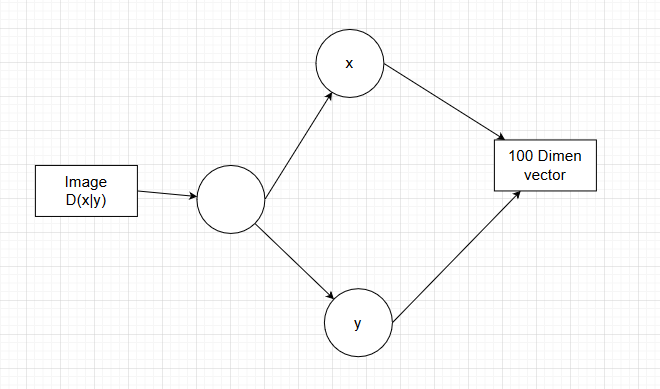
\includegraphics[width=4cm]{figures/1174096/tugas9/teori5.PNG}
		\caption{Ilustrasi discriminator network AgecGAN}
	\end{figure}

	\item Jelaskan dengan ilustrasi gambar apa itu pretrained Inception-ResNet-2 Model.
	\hfill\break
	Inception Resnet 2 model pre trained merupakan sebuah package untuk mendefinisikan, melatih, dan mengevaluasi sesuai dengan checkpoint dan definisi model untuk beberapa network pada klasifikasi gambar.
	\begin{figure}[H]
	    \centering
	    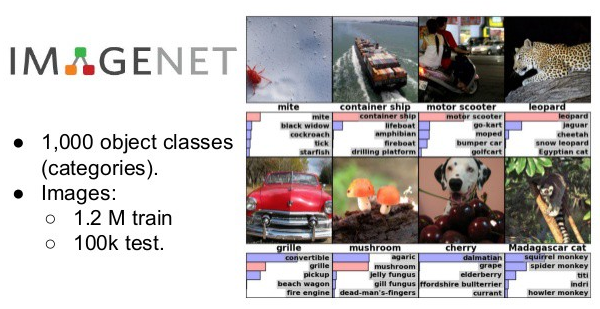
\includegraphics[width=4cm]{figures/1174096/tugas9/teori6.PNG}
	    \caption{Ilustrasi pretrained Inception-ResNet-2 Model}
    \end{figure}

    \item  Jelaskan dengan ilustrasi gambar sendiri arsitektur Face recognition network Age-cGAN.
    \hfill\break
    Face Recognition network Age-cGAN digunakan untuk dapat mengenali identitas seseorang dalam gambar yang diberikan
    \begin{figure}[H]
	    \centering
	    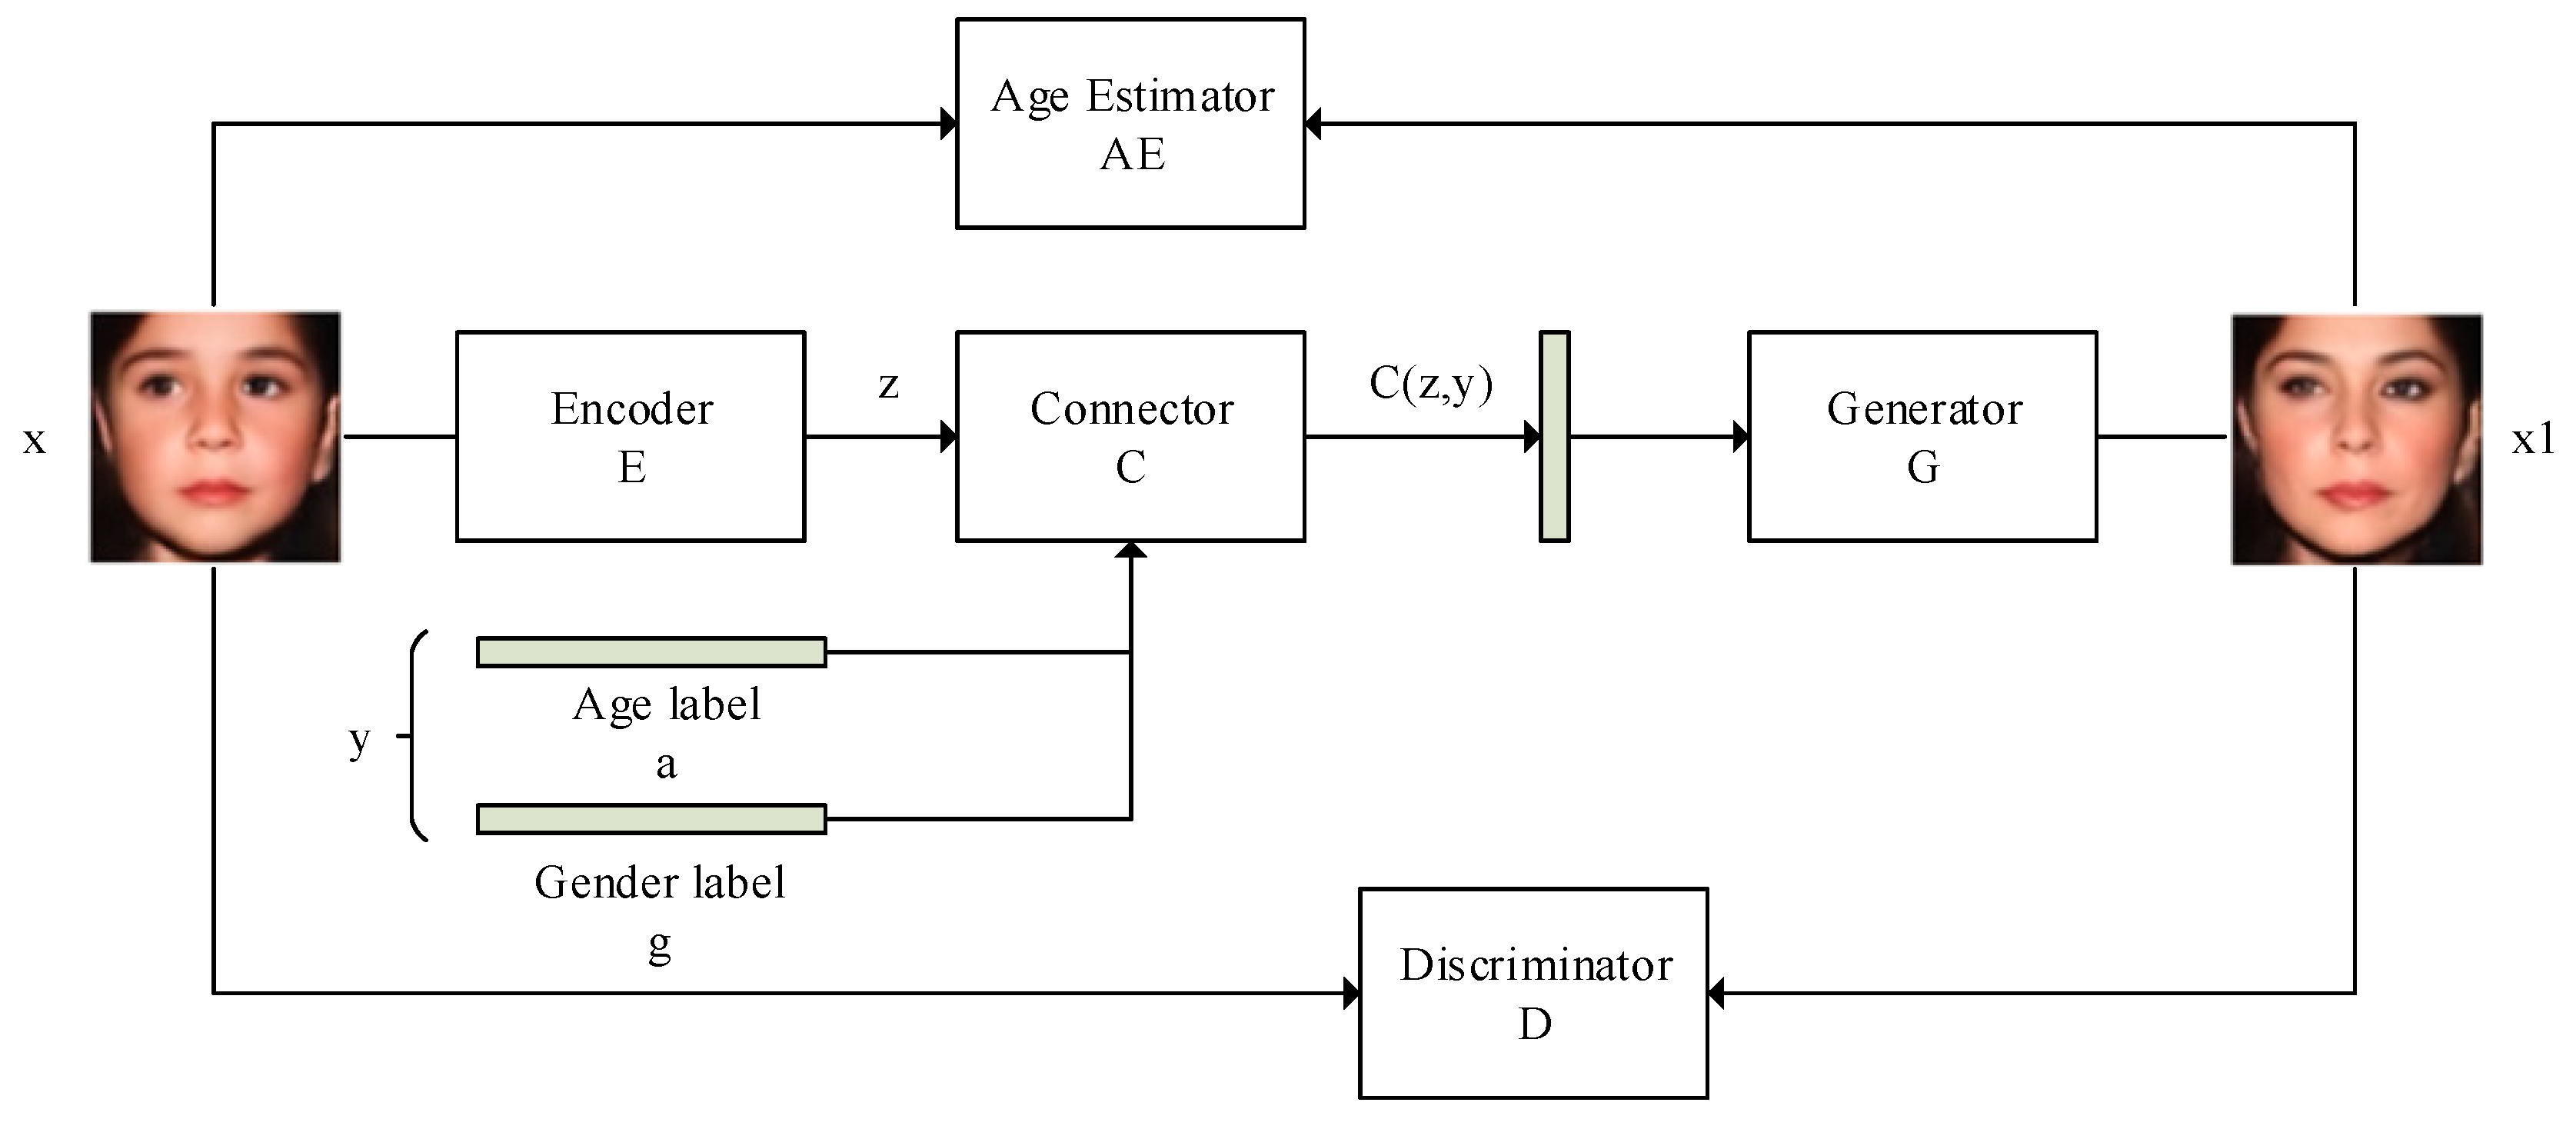
\includegraphics[width=4cm]{figures/1174096/tugas9/teori7.PNG}
	    \caption{ilustrasi arsitektur Face recognition network Age-cGAN}
    \end{figure}

    \item Sebutkan dan jelaskan serta di sertai contoh-contoh tahapan dari Age-cGAN
    \hfill\break
    Age-cGAN memiliki beberapa tahapan pelatihan. Age-cGAN memiliki empat jaringan, yang dilatih dalam tiga tahap. Pelatihan AgecGAN terdiri dari tiga tahap:

	\begin{itemize} 
			\item pelatihan GAN bersyarat: pada tahap ini, kita melatih jaringan Generator dan jaringan diskriminator.
    		\item awal pendekatan vektor laten: pada tahap ini, kami melatih jaringan Encoder.
    		\item optimasi vektor laten: pada tahap ini, kami mengoptimalkan kedua encoder dan jaringan generator.
		\end{itemize}

    \item Berikan contoh perhitungan fungsi training objektif
    \hfill\break
    Objektif Trainning ialah untuk meminimalkan loss function sebagai log likelihood function yang diberikan pada persamaan dimana D melambangkan trainning data.
    \begin{figure}[H]
	    \centering
	    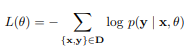
\includegraphics[width=4cm]{figures/1174096/tugas9/teori9.PNG}
	    \caption{ilustrasi perhitungan fungsi training objektif}
    \end{figure}
    

    \item Berikan contoh dengan ilustrasi penjelasan dari Initial latent vector approximation
    \hfill\break
    Latent Vector Aproximation adalah metode untuk memperkirakan vektor laten untuk mengoptimalkan rekonstruksi gambar wajah. Untuk memperkirakan vektor laten, kami memiliki jaringan Encoder. Kami melatih jaringan Encoder pada gambar yang dihasilkan dan gambar nyata. Setelah dilatih, Jaringan Encoder akan mulai menghasilkan vektor laten dari Distribusi. Tujuan pelatihan fungsi untuk pelatihan jaringan Encoder adalah kehilangan jarak Euclidean.
    \begin{figure}[H]
	    \centering
	    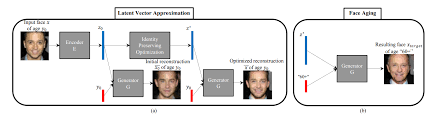
\includegraphics[width=4cm]{figures/1174096/tugas9/teori10.PNG}
	    \caption{ilustrasi Initial latent vector approximation}
    \end{figure}

    \item Berikan contoh perhitungan latent vector optimization
    \hfill\break
    Perhitungan lantent optimization menggunakan metode yang relatif sederhana, tergantung pada jumlah kecil parameter yang diperlukan, sehingga pada latent optimization dapat memetakan setiap gambar x dari dataset ke vektor acak dimensi rendah zi dalam ruang laten z.
    \begin{figure}[H]
	    \centering
	    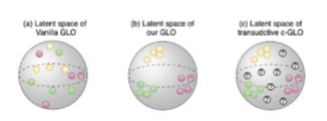
\includegraphics[width=4cm]{figures/1174096/tugas9/teori11.PNG}
	    \caption{ilustrasi perhitungan latent vector optimization}
    \end{figure}

\end{enumerate}

\subsection{Praktek Program}
\begin{enumerate}
	\item  Jelaskan bagaimana cara ekstrak file dataset Age-cGAN menggunakan google colab
    \hfill\break
    Cara yang dilakukan untuk ekstraksi file melalui google colab yaitu dengan mengopy path dari file yang telah ada di drive kedalam code ekstraksi
    \lstinputlisting[firstline=8, lastline=11]{src/1174096/9/1174096.py}
	
	\item  Jelaskan bagaimana kode program bekerja untuk melakukan load terhadap dataset yang sudah di ekstrak, termasuk bagaimana penjelasan kode program perhitungan usia
    \hfill\break
    Dalam melakukan load dataset yang telah diekstrak, terdapat beberapa proses, yaitu melakukan load file wiki.mat. Setelah itu melakukan load list file. Kemudian list serial number matlab, tahun pengambilan foto. Lalu mengkalkulasikan umur. setelah itu membuat list tuple, lalu mereturn list semua gambar dan perkiraan umur.
    \lstinputlisting[firstline=13, lastline=38]{src/1174096/9/1174096.py}
    
    
	\item  Jelaskan bagaimana kode program The Encoder Network bekerja dijelaskan dengan bahasa awam dengan ilustrasi sederhana
    \hfill\break
    Proses Encoder berfungsi untuk mempelajari pemetaan terbalik dari gambar wajah dan kondisi usia dengan vector latent Z.
	\lstinputlisting[firstline=40, lastline=80]{src/1174096/9/1174096.py}
	

	\item Jelaskan bagaimana kode program The Generator Network bekerja dijelaskan dengan bahasa awam dengan ilustrasi sederhana
    \hfill\break
    Proses Generator agar bekerja dengan baik dibutuhkan representasi dari gambar wajah dan vector kondisi sebagai inputan yang menghasilkan sebuah gambar.
    \lstinputlisting[firstline=82, lastline=121]{src/1174096/9/1174096.py}

	\item Jelaskan bagaimana kode program The Discriminator Network bekerja dijelaskan dengan bahawa awam dengan ilustrasi sederhana
    \hfill\break
    Proses Discriminator untuk membedakan antara gambar asli dan gambar palsu.
    \lstinputlisting[firstline=123, lastline=155]{src/1174096/9/1174096.py}

	\item Jelaskan bagaimana kode program Training cGAN bekerja dijelaskan dengan bahasa awam dengan ilustrasi sederhana
    \hfill\break
    Proses Training cGAN ini dengan load file .mat pada dataset lalu epoch sebanuak 500 kali.
    \lstinputlisting[firstline=157, lastline=174]{src/1174096/9/1174096.py}
	
	\item Jelaskan bagaimana kode program Initial dan latent vector approximation bekerja dijelaskan dengan bahawa awam dengan ilustrasi sederhana
    \hfill\break
    Initial dan Latent Vector Approximation bekerja melakukan predicsi epoch yang telah di buat sebanyak 500 kali, dan nanti hasilnya ada di folder result.
    \lstinputlisting[firstline=176, lastline=224]{src/1174096/9/1174096.py}
\end{enumerate}

\subsection{Penanganan Error}
\begin{enumerate}
	\item IndentationError: unexpected indent
	\begin{figure}[H]
		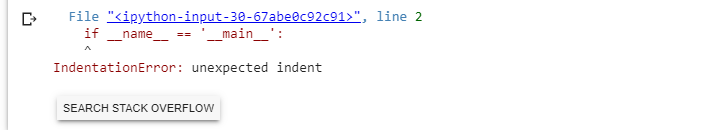
\includegraphics[width=4cm]{figures/1174096/tugas9/error.PNG}
		\centering
		\caption{IndentationError}
	\end{figure}
	\item Tuliskan Kode Error dan Jenis Error
	\begin{itemize}
		\item IndentationError
	\end{itemize}
	\item Cara Penangan Error
	\begin{itemize}
		\item IndentationError
		\hfill\break
		Error terjadi karena indentasi atau letak kode berada di posisi yang tidak seharusnya. cara untuk mengatasi error tersebut adalah dengan memperbaiki posisi indentasi kode sesuai dengan penulisan kode python yang benar.
	\end{itemize}
\end{enumerate}

\subsection{Bukti Tidak Plagiat}
\begin{figure}[H]
\centering
	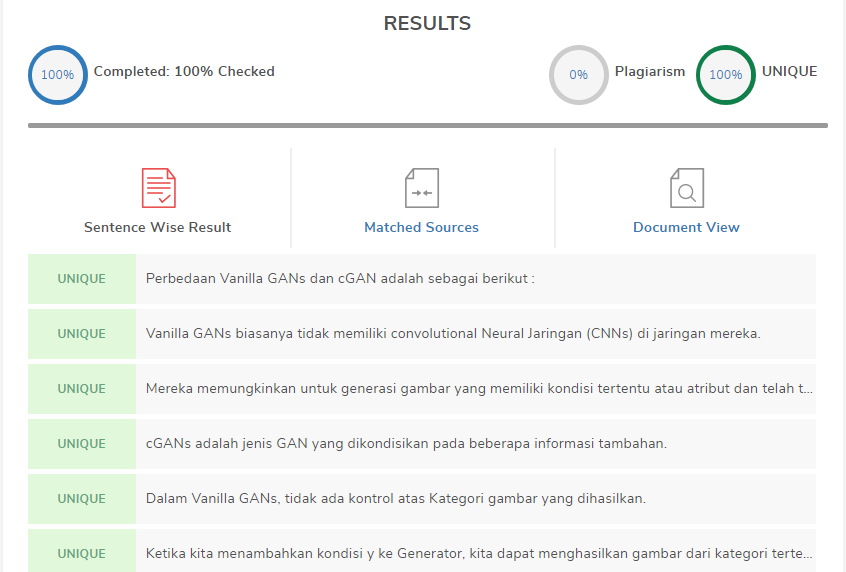
\includegraphics[width=4cm]{figures/1174096/tugas9/plagiarisme.PNG}
	\caption{Bukti Tidak Melakukan Plagiat Chapter 9}
\end{figure}
